\documentclass[pdf,colorBG,slideColor]{prosper}
\hypersetup{pdfpagemode=FullScreen}

\usepackage{amsmath}
\usepackage{graphicx}

\title{THOR}
\subtitle{Tree High Order Reduce}
\author{Garrett Boyer, Ryan Riegel, Alexander Gray}
\institution{College of Computing\\Georgia Institute of Technology}

\newcommand{\itemt}[1]{\item {\bf #1} -}


\newcommand{\authornote}[1]{\footnote{Note to self: #1}}
\newcommand{\authorsnote}[1]{\authornote{#1}}
\newcommand{\com}[1]{{\small \textit{((#1))}}}

\newcommand{\union}{\cup}
\newcommand{\intersect}{\cap}
\newcommand{\Union}{\bigcup}
\newcommand{\Intersect}{\bigcap}
\newcommand{\bigvec}[1]{\mathop{\overrightarrow{#1}}}

\newcommand{\otimeshat}{\widehat{\otimes}}
\newcommand{\odothat}{\widehat{\odot}}

\newcommand{\prefsplit}[2]{#1 \succ #2}
\newcommand{\summary}{\hat{\sigma}}

\DeclareMathOperator*{\map}{map}
\DeclareMathOperator*{\worst}{worst}
\DeclareMathOperator*{\argmin}{argmin}
\DeclareMathOperator*{\argmax}{argmax}
\DeclareMathOperator{\TWOPT}{TWOPOINT}
\DeclareMathOperator{\cardinality}{cardinality}
\DeclareMathOperator{\hrect}{hrect}
\DeclareMathOperator{\child}{child}
\DeclareMathOperator{\visited}{visited}
\DeclareMathOperator{\unvisited}{unvisited}
\DeclareMathOperator{\prune}{prune}
\DeclareMathOperator{\IF}{if}
\DeclareMathOperator{\ATDISCRETION}{}

\newcommand{\fig}[1]{Figure~\ref{fig:#1}}

\newcommand{\Gnp}{\Psi}
\newcommand{\gnp}{\psi}

%\newcommand{\psty}{\scriptstyle}
\newcommand{\psty}{}
\newcommand{\X}{\\ \psty}
\newcommand{\x}{\X \hspace{0.13in}}
\newcommand{\xx}{\X \hspace{0.26in}}
\newcommand{\xxx}{\X \hspace{0.39in}}
\newcommand{\xxxx}{\X \hspace{0.52in}}

\newcommand{\defterm}[1]{{\bf #1}}
\newcommand{\nbody}{$N$-body}

\newcommand{\kdroot}[1]{#1^{\text{root}}}
\newcommand{\kdleft}[1]{#1^{\!L}}
\newcommand{\kdright}[1]{#1^{\!R}}
\newcommand{\kdparent}[1]{#1^{\!P}}

\newcommand{\lo}[1]{#1^{l}}
\newcommand{\up}[1]{#1^{u}}
\newcommand{\distlo}{\lo{d}}
\newcommand{\distup}{\up{d}}
\newcommand{\dist}[2]{d(#1,#2)}

%\newcommand{\myOp}[1]{\mathop{\bigotimes\nolimits\hspace{-0.045in}_{#1}}}
\newcommand{\nameOp}[2]{\mathop{#1\nolimits\!\!_{#2}}}
\newcommand{\nameop}[2]{{\scriptstyle\:}#1_{\!#2}}
\newcommand{\myOp}[1]{\nameOp{\bigotimes}{#1}}
%\newcommand{\myop}[1]{\otimes\hspace{-0.04in}_{#1}\hspace{0.03in}}
\newcommand{\myop}[1]{\nameop{\otimes}{#1}}
\newcommand{\myOutop}[1]{\nameOp{\bigodot}{#1}}
\newcommand{\myoutop}[1]{\nameop{\odot}{#1}}

\newcommand{\letterglob}{\psi}
\newcommand{\outglob}{\Psi}
\newcommand{\inglob}{\psi}
\newcommand{\Opglob}{\myOp{\letterglob}}
\newcommand{\opglob}{\myop{\letterglob}}
\newcommand{\fglob}{f_{\!\letterglob}}
\newcommand{\gglob}{g_{\!\letterglob}}
\newcommand{\canpruneglob}{C_{\!\letterglob}}
\newcommand{\deltaglob}{\summary_{\!\letterglob}}

\newcommand{\letterqr}{\rho}
\newcommand{\outqr}{\varrho}
\newcommand{\inqr}{\rho}
\newcommand{\Opqr}{\myOp{\letterqr}}
\newcommand{\opqr}{\myop{\letterqr}}
\newcommand{\fqr}{f_{\!\letterqr}}
\newcommand{\gqr}{g_{\!\letterqr}}

\newcommand{\letterqrv}{\vec{\rho}}
%\newcommand{\outqrv}{\vec{\rho}}
\newcommand{\inqrv}{\vec{\rho}}
%\newcommand{\fqrv}{f_{\letterqrv}}
%\newcommand{\gqrv}{g_{\letterqrv}}
\newcommand{\deltaqrv}{\summary_{\!\letterqrv}}
\newcommand{\canpruneqrv}{C_{\!\letterqrv}}
\newcommand{\identqr}{0_{\!\letterqrv}}
\newcommand{\varqrv}{\letterqrv^{\:C\!}}
\newcommand{\varqrvparent}{\letterqrv^{\:P\!}}

\newcommand{\lettermu}{\mu}
%\newcommand{\inmu}{\mu}
\newcommand{\inmu}{\mu}
\newcommand{\Outopmu}{\widehat{\nameOp{\bigodot}{\lettermu}}}%\mathop{\widehat{\bigodot\nolimits}\!\scriptstyle{\mu}}}
\newcommand{\outopmu}{\:\widehat{\odot}_{\!\mu}\:}
\newcommand{\Opmu}{\myOp{\lettermu}}
\newcommand{\opmu}{\myop{\lettermu}}
\newcommand{\fmu}{f_{\!\lettermu}}
\newcommand{\fmuv}{\vec{f_{\!\lettermu}}}
\newcommand{\deltamu}{\summary_{\!\lettermu}}
\newcommand{\canprunemu}{C_{\!\lettermu}}
\newcommand{\heurqr}{H}
\newcommand{\identmu}{0_{\lettermu}}
\newcommand{\varmuchild}{\lettermu^{\!C}}
\newcommand{\varmuparent}{\lettermu^{\!P}}

%\newcommand{\muparent}{\inmu_{\text{coarse}}}
%\newcommand{\muchild}{\inmu_{\text{children}}}
%\newcommand{\muvisit}{\inmu_{\text{visited}}}
%\newcommand{\muall}{\inmu_{\text{all}}}

%\newcommand{\hatpi}{\hat{\outpi}}
%\newcommand{\piparent}{\outpi_{\text{parent}}}

\newcommand{\letterstat}{s}
\newcommand{\namestat}[1]{\sigma_{\text{#1}}}
\newcommand{\outstat}{\sigma}
\newcommand{\instat}{s}
\newcommand{\Opstat}{\myOp{\letterstat}}
\newcommand{\opstat}{\myop{\letterstat}}
\newcommand{\fstat}{f_{\!\letterstat}}
\newcommand{\gstat}{g_{\!\letterstat}}

% Affinity propagation


\newcommand{\eqspace}{\!\!\!\!}
\newcommand{\true}{\text{true}}
\newcommand{\ocpos}[1]{c^{+}_{#1}}
\newcommand{\ocneg}[1]{c^{-}_{#1}}
\newcommand{\cpos}[2]{\ocpos{#1 \neq #2}}
\newcommand{\cneg}[2]{\ocneg{#1 \neq #2}}

\newcommand{\respo}[2]{R_{#1#2}}
\newcommand{\avail}[2]{A_{#1#2}}
\newcommand{\simil}[2]{S_{#1#2}}

\newcommand{\vecrho}{\vec{\rho}}
\newcommand{\vecalpha}{\vec{\alpha}}
\newcommand{\frho}[1]{\rho_{#1}}
\newcommand{\falpha}[1]{\alpha_{#1}}
\newcommand{\falphaj}[2]{\alpha_{#1[#2]}}

\newcommand{\falphamax}{\alpha^{u}}
\newcommand{\falphamin}{\alpha^{l}}
\newcommand{\frhomax}{\rho^{u}}
\newcommand{\frhomin}{\rho^{l}}

\newcommand{\alphacand}{v}



\begin{document}

\maketitle

\begin{slide}{Mission}
  Allow mainstream algorithm developers to create well-tuned parallel
  dual-tree algorithms.

  \begin{itemize}
    \itemt{Motivation}
    Multi-tree algorithms are asymptotically fastest at many problems.
    Parallelization allows even greater scalability.
    \itemt{Approach}
    \begin{enumerate}
      \item Generalize the multi-tree problem space.
      \item Parallelize the generalized problem.
    \end{enumerate}
  \end{itemize}
  % Introduction, Motivation
  % What is the point?
  % Why am I presenting? To explain THOR.
  % Why am I creating THOR? To parallelize dual-tree algorithms.
  % My audience has no idea that these tree algorithms can be generalized.
  % Keep this in mind -- it's interesting to them.
\end{slide}

\begin{slide}{Dual-Tree Algorithms - Intro}
  \begin{itemize}
    \itemt{Cartesian Hierarchy}
    Hierarchically divide the Cartesian product of two
    datasets to perform an all-pairs computation.
    \itemt{Trees}
    Use existing spatial trees to divide each dataset.
    \itemt{Pruning}
    Exploration can stop on subcomponent $X \times Y$ if we know a suitable
    result for it, or if its result doesn't affect the overall computation.
    (More on this later.)
    \itemt{Data Intensive}
    Dual-tree algorithms are fundamentally data intensive -- operating on
    lots of data, and moreover, all data pairs.
    This data intensive nature is the core issue in dual-tree parallelization.
  \end{itemize}
\end{slide}

\begin{slide}{Dual-Tree Algorithms - Example}
  \begin{itemize}
    \itemt{Two-Point Correlation}
    Number of pairs within radius $h$.
    \[\sum_{x \in X} \sum_{y \in X} I(d(x, y) \leq h)\]
    \itemt{Nearest Neighbors}
    For each query $q \in Q$, find the nearest $r \in R$.
    \[\map_{q \in Q} \argmin_{r \in R} d(q,r)\]
    \itemt{Kernel Density Estimation}
    For each query $q \in Q$, find a kernel sum generated around points $r \in R$.
    \[\map_{q \in Q} \sum_{r \in R} K(q, r)\]
  \end{itemize}
\end{slide}

\begin{slide}{Physical $N$-Body Problem}
  \begin{itemize}
    \itemt{Problem}
    Simulate a system of particles that exert mutual force.
    Find particle's position at a later time.
    \itemt{Barnes-Hut Algorithm}
    Create an oct-tree.
    For each query particle, traverse the oct-tree, approximating the force
    of distant particles. O(N log N).
    \itemt{Fast Multipole Method}
    Create an oct-tree.
    Bottom-up, compute multipole expansions.
    Top-down, aggregate siblings' expansions.
    Compute per-particle force using the expansions.
    O(N).
  \end{itemize}
  % The problem
  % BH
  % FMM and AFMM
\end{slide}

\begin{slide}{Software Frameworks}
  \begin{itemize}
    \itemt{Frameworks}
    Software frameworks execute a generalized problem, where
    users fill in the blanks.
    \itemt{Map-Reduce}
    Map-Reduce runs problems that involve a step of preprocessing and
    further aggregation.
    It solves problems like creating a reverse-index, counting words
    in documents, and much more.
    \itemt{Premise}
    If a problem is generalizable, then create an implementation that
    has certain provable properties.
    All members of the problem space therefore inherit those properties.
  \end{itemize}
\end{slide}

\begin{slide}{Software Frameworks - Alternatives}
  Why frameworks?  Consider some alternatives:
  \begin{itemize}
    \itemt{Parallel Languages}
    UPC provides parallel extensions to C.  NESL is a parallel ML-like
    language.
    \\ {\bf Con:} Little control over implementation details.
    \itemt{Virtual Memory}
    Some projects simulate virtual memory over multiple computers
    using page tables.
    \\ {\bf Con:} Makes worst-case assumptions about semantics.
    Dual-tree algorithms have much less strict requirements.
    \itemt{Hand Parallelization}
    $N$-body methods have been hand-parallelized for decades in a way that
    is impossible for other approaches to compete with.
    \\ {\bf Con:} Takes months, and we'll show this work is avoidable.
  \end{itemize}
\end{slide}

\begin{slide}{GNP Basics}
  Unlike many software frameworks, ours is inherently mathematical.

  Next, we dive into the formalisms behind our framework.
\end{slide}

\begin{slide}{GNP Basics - Notation}
  \begin{itemize}
    \itemt{Map Operator} $\map$ builds a list of results.
    Mathematically, $\map$ outputs a set of key-value pairs.
    \itemt{Generic Operators} $\bigodot, \bigotimes$ mean {\em any} commutative, associative operator.
    \itemt{Trees} A tree node {\em summarizes} a set of points.
    $\kdroot{X}$ is the entire data set.
    $X$ is a subset with parent $\kdparent{X}$,
    partitioned into children $X = \kdleft{X} \union \kdright{X}$.
    \itemt{Generic Statistics} $\outstat(X)$ is a statistic on a set of points,
    such as bounding box, mean, or variance.
    \itemt{Upper/Lower Bounds} $\distup(\outstat(X), \outstat(Y))$ is an upper-bound distance
    between bounding boxes.  $\distlo$ is the lower-bound.
  \end{itemize}
\end{slide}

\begin{slide}{GNP Basics - Reduce Problem}
  A \defterm{second-order reduce problem} solves for dataset pair $X, Y$:
    \[\begin{array}{l}
      \displaystyle \gnp(X, Y) = \bigodot_{x \in X} g\!\left(x, \bigotimes_{y \in Y} f(x, y) \right)
    \end{array}\]
  for commutative, associative operators $\bigodot, \bigotimes$, and user-provided
  outer function $g$ and inner function $f$.
  \\
  A Generalized $N$-body problem (GNP) additionally requires that, for any partitioning $\kdleft{Y} \union \kdright{Y} = Y$:
    \[\begin{array}{ll}
     \gnp(X,Y) = \gnp(\kdleft{X}, Y) \odot \gnp(\kdright{X},Y) & \text{\it commutative, associatve}
     \\
     \gnp(X,Y) = \gnp(X,\kdleft{Y}) \otimes \gnp(X,\kdright{Y}) & \text{\it block decomposition}
    \end{array}\]
\end{slide}

\begin{slide}{GNP Basics - Expansion and Pruning}
  \begin{itemize}
    \itemt{Expansion}
    Consider expression $\gnp(\kdroot{X}, \kdroot{Y})$.
    Replace any term with its decomposition.
    Repeat until explosion.
    \itemt{Intrinsic Prune}
    Substitute subexpressions whose values can be determined with
    in-tree statistics.
    \begin{itemize}
      \itemt{Example: Two-point correlation} The nodes' bounding boxes are
      farther apart than radius $h$.
    \end{itemize}
    \itemt{Extrinsic Prune}
    A subexpression's value is determined to be "good enough".
    Checked via tree node statistics AND summaries of surrounding computations.
    \begin{itemize}
      \itemt{Example: Nearest neighbors}
      The nodes' bounding boxes are farther apart than the
      worst-case candidate neighbor.
    \end{itemize}
  \end{itemize}
\end{slide}

\begin{slide}{Q/R Problems}
  \begin{itemize}
    \itemt{Definition} A \defterm{query-reference} problem has $\bigodot = \map$, i.e. one result per query.
    \itemt{Universality} {\it Any} second-order reduce problem can be transformed into a query-reference problem.
    \begin{itemize} \item
      Replace outer operator with $\map$, and treat original operator as a postprocess step.
    \end{itemize}
  \end{itemize}
  Next, we'll focus on solving these problems formally.
\end{slide}

\begin{slide}{Q/R Problems - Formalization}
  Assume commutative, associative $\opqr$.
  For each query $q$, solve $\outqr(q, \kdroot{R})$, given:
  \begin{eqnarray*}
    \outqr(q, R) &\equiv& \gqr(q, \inqr(q, R)),
x    \\
    \inqr(q, R) &\equiv& \Opqr_{r \in R} \fqr(q, r).
  \end{eqnarray*}
  Sometimes, the same \defterm{mass result} $\inqrv(Q, R)$
  applies to many queries for a particular reference node.
  This is a prune, formally expressed,
  \[
  \forall q \in Q,~~ \inqr(q, R) \gets \inqrv(Q, R).
  \]
\end{slide}

\begin{slide}{Q/R Problems - Solving}
  We may compute $\inqrv$ using the three rules:
  \[\begin{array}{l}
    \inqrv(Q, R) = \inqrv(Q, \kdleft{R}) \opqr \inqrv(Q, \kdright{R}),
    \\
    \text{if prune occurs for } \kdparent{Q} \supset Q \text{, then } \inqrv(Q, R) = \inqrv(\kdparent{Q}, R),
    \\
    \text{if } \canpruneqrv(\outstat(Q), \outstat(R)) \text{, then } \inqrv(Q, R) = \deltaqrv(\outstat(Q), \outstat(R)).
  \end{array}\]
  We have:
  \begin{itemize}
    \itemt{$\canpruneqrv$} An intrinsic prune check.
    \itemt{$\deltaqrv$} The pruned value, computed with summary statistics.
  \end{itemize}
\end{slide}

\begin{slide}{Q/R Problems - Example}
  Range count is a query-reference analog of two-point correlation,
  \[\map_{q \in Q} \sum_{r \in R} I(\dist{q}{r} < h).\]
  A THOR user simply implements the following in C++.
  \begin{eqnarray*}
  \gqr(q, \inqr) &\equiv& \inqr
  \\
  \opqr &\equiv& +
  \\
  \fqr(q,r) &\equiv& I(\dist{q}{r} < h)
  \\
  \canpruneqrv(\sigma(Q), \sigma(R))
  &\equiv&
  \begin{array}{l}\distup(\outstat(Q),\outstat(R)) < h \\ \vee \distlo(\outstat(Q),\outstat(R)) \geq h\end{array}
  \\
  \deltaqrv(\outstat(Q),\outstat(R)) &\equiv& \left\{ \begin{array}{l} 0 \text{ if } \distup(\outstat(Q),\outstat(R)) < h \\ |R| \text{ if } \distlo(\outstat(Q),\outstat(R)) \geq h \end{array}\right.
  \end{eqnarray*}
\end{slide}

\begin{slide}{Q/R Problems - Extrinsic Pruning}
  \vspace{-.1in}
  \begin{itemize}
    \item We compute \defterm{query summary results} $\inmu(Q, \kdroot{R})$
    to achieve extrinsic pruning for query node $Q$.
    The \defterm{ideal} value bounds the exact results of each query,
      \begin{equation*}
      \inmu(Q, R) \gets \Outopmu_{q \in Q} \fmu(q, \inqr(q, R)).
      \end{equation*}
    During computation, we make pessimistic bounds using only
    summary statistics and completed computations.
    \item Extrinsic prunes use a separate prune check $\canprunemu(\outstat(Q), \outstat(R), \inmu(Q, \kdroot{R}))$.
    \item The subjective \defterm{quality} of $\lettermu$ reflects how
    closely it approaches the ideal value.
    Higher-quality values aid pruning.
    \item Computational details omitted for brevity.
  \end{itemize}
\end{slide}

\begin{slide}{Q/R Problems - Conclusion}
  \begin{itemize}
    \itemt{Generality}
    We maintain that our query-reference model can solve all second-order reduce problems.
    Whether a problem can be solved efficiently is up to pruning rules and the execution pattern.
    \itemt{Execution}
    The aforementioned ``rules'' have few constraints on their execution.
    Depth-first, breadth-first, and importantly {\em parallel} expansion patterns are fair game!
  \end{itemize}
  
  We'll now focus on parallel executions.
\end{slide}

\begin{slide}{Work Decomposition}
  \begin{itemize}
    \itemt{Two Axes}
    A dual-tree problem can theoretically be decomposed both query and reference trees.
    \itemt{Query Only}
    We decompose by dividing the query tree only:
    \begin{itemize}
      \itemt{Private Data}
      No writes to shared data.
      \itemt{Quality of $\lettermu$}
      For high-quality query summary results, one must consider all references.
      Considering referenes independently makes this problematic.
      \itemt{Scheduling}
      Distant query-reference pairs complete orders of magnitude faster than
      nearby ones.
      Unpredictable runtimes unduly complicates scheduling.
    \end{itemize}
  \end{itemize}
\end{slide}

\begin{slide}{Work Decomposition - An Item}
  \begin{itemize}
    \item A \defterm{work item} is a query node that is solved with a standard
    serial expansion pattern.
    \item We'll address the topic of decomposition two more times.
  \end{itemize}
\end{slide}

\begin{slide}{Communication}
  \begin{itemize}
    \itemt{Fundamental Issue} Communication is a fundamental issue of parallel programming.
    \itemt{Limiting Factor} Decades of experience show communication is the prime
    limiting factor in parallel $N$-body methods.
    \itemt{Essential Trees} Although writes are independent, many reference
    points and tree nodes may be needed to perform a computation.  These are
    the \defterm{essential} points and nodes for a particular query node.
  \end{itemize}
  % Introduce Domain Decomposition here
\end{slide}

\begin{slide}{Comm. - Decompositions}
  \begin{itemize}
    \itemt{Domain Decompositions}
    A domain decomposition divides queries among processors.
    \itemt{Goal}
    One attempts to minimize locally essential trees, by maximizing
    overlap between queries owned by a processor.
    \itemt{Past Techniques}
    Neglecting scheduling details, we consider previous work:
    \begin{itemize}
      \itemt{ORB Tree} A $kd$-tree balanced by estimated work divides
      points hierarchically among processors.
      \itemt{Cost-Zones} Distribute points based on contiguous regions of
      the Barnes-Hut tree traversal.
    \end{itemize}
    \itemt{THOR's Technique}
    We combine the two by building the underlying $kd$-tree with
    the domain decomposition in mind.
  \end{itemize}
\end{slide}

\begin{slide}{Comm. - Approach}
  \begin{itemize}
    \item We summarize previous approaches for $N$-body communication:
    \begin{itemize}
      \itemt{Sender Initiated}
      Compute locally essential trees beforehand and send in one large pass.
      {\bf Con}: Computing these trees is problem-specific.
      \itemt{Use Shared Memory}
      J. Singh argues you should just use large NUMA system.
      {\bf Con}: NUMA systems are very expensive.
      \itemt{Use Blocks}
      Divide data and nodes into blocks, and request blocks on demand.
      Similar to underlying NUMA systems, and allows disk-based algorithms.
    \end{itemize}
    \item We use blocks.  Blocked methods are adaptive, have attractive
    performance, and naturally allow disk-based trees.
    Salmon and Warren successfully tried this a decade ago!
  \end{itemize}
\end{slide}

\begin{slide}{Comm. - Distributed Cache}
  \begin{itemize}
    \itemt{Cached Array}
    A cached array is distributed among machines block-by-block.
    One cache one for points, one for nodes.
    \itemt{Replication}
    Blocks are stored on all machines that need it, but maintained by only one.
    All machines have the directory.
    \itemt{Consistency}
    Global consistency is maintained only at infrequent sync points, once per GNP.
    Between sync points, THOR writes to explicitly declared disjoint contiguous regions.
    \itemt{Software Cache}
    Blocks are accessed by explicitly locking and unlocking pages.
    An unlocked page is placed in a queue for potential eviction.
    Out-of-core blocks are requested from disk or other machines.
  \end{itemize}
\end{slide}
  
\begin{slide}{Comm. - Distributed Cache}
  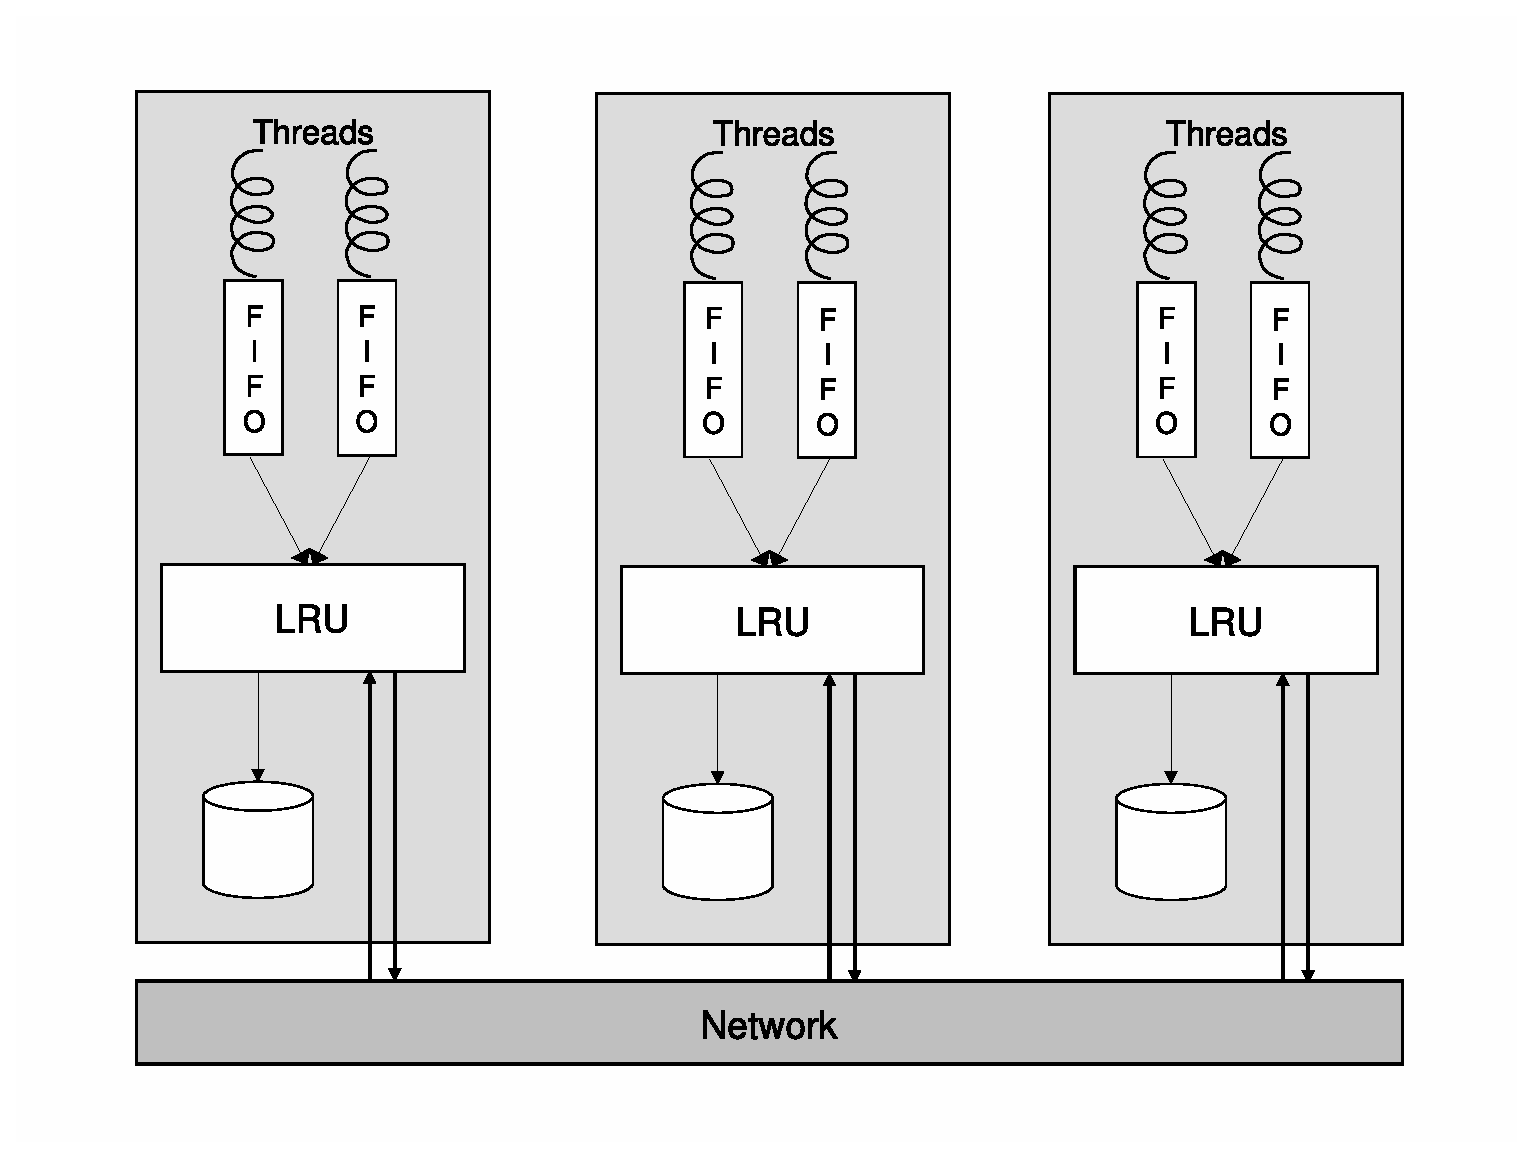
\includegraphics[width=4.0in]{DistributedArchitecture.eps}
\end{slide}

\begin{slide}{Comm. - Data Layout}
  \begin{itemize}
    \itemt{Point Order}
    Points are stored in perfect left-to-right tree order.
    For $kd$-trees, this is analagous to a Morton ordering.
    \itemt{Point Blocking}
    Each block of points corresponds to one tree node.
    The tree-builder makes block-aligned splits until a single block
    is reached, then performs midpoint splits.
    \itemt{Node Order}
    Previous work shows both pre-order and high-fanout orderings work well
    for dual-tree algorithms. We use pre-order because it allows contiguous
    groupings of nodes.
  \end{itemize}
\end{slide}

\begin{slide}{Scheduling}
  \begin{itemize}
    \itemt{Objective}
    Assign tasks to processors to minimize overall run time, keeping in mind
    the ``weakest link'' principle.
    \itemt{Past Techniques}
    The aforementioned ORB and cost-zones techniques require work estimates
    per query from previous iterations.
    Unfortunately, THOR cannot generally assume multiple iterations, though
    future work can take this into account.
    \itemt{Dynamic Scheduling}
    THOR must use a dynamic scheduler to account for unforseen load imbalances.
    In practice, very simple dynamic schedulers achieve good performance.
  \end{itemize}
\end{slide}

\begin{slide}{Scheduling in THOR}
  An overview of THOR's scheduler:
  \begin{itemize}
    \itemt{Initial Assignment}
    Divide query tree into nodes smaller than a processor is expected to handle.
    Create an initial task decomposition based on the domain decomposition.
    \itemt{Assignment Process}
    A thread requests a work item from the master whenever it becomes idle.
    Threads from the same machine are treated identically.
    \itemt{Overflow}
    If a machine completes its work, the spatially closest unfinished work
    item is assigned.
  \end{itemize}
\end{slide}

\begin{slide}{Scheduling - Further Work}
  THOR's primitive scheduler works well, but it could be better:
  \begin{itemize}
    \itemt{Restart} For pathological imbalances, a work item taking unusually
    long should be restarted and distributed among processors.
    \itemt{Distributed Assignment} Centralized scheduling becomes a bottleneck
    as the number of processors grows larger.
    \itemt{Hierarchical Redistribution} Rather than a greedy overflow policy
    that doesn't optimize for holistic locality, overflow can be
    handled by aggressively reassigning large chunks of work to large chunks
    of processors.
  \end{itemize}
\end{slide}

% QUESTION: Separate Setup/Results/Discussion sections?

\begin{slide}{Experiments}
  Our experiments must be {\em realistic}:
  \begin{itemize}
    \itemt{Application} Our experiments must apply to problems someone
    might want to solve.  Finding nearest neighbors on uniform data is
    silly -- just use a grid!
    \itemt{Necessity}
    A problem that takes a few minutes on one processor probably
    doesn't need to be parallel.
    If it's an hour on one processor, 128 processors is too many - consider
    the bureaucratic red tape invovled.
  \end{itemize}
  We'll look at problems that are too large to be solved practically on
  a single processor.
\end{slide}

\begin{slide}{Experiments - Setup}
  % algorithms and data-sets
  Data:
  \begin{itemize}
    \itemt{Speech}
    12-dimensional, frequency-domain, with manifold.
    Nearest neighbors and KDE.
    \itemt{Galaxy}
    3-d positions of galactic halos ($\Lambda CDM$).
    Two-point correlation.
    \itemt{Redshift}
    4-dimensional redshift data for quasar detection.
    KDE.
  \end{itemize}
  We run KDE with Gaussian kernel and finite difference method.
\end{slide}

\begin{slide}{Experiments - Overhead}
  Two sources of potential overhead studied.
  \begin{itemize}
    \itemt{Infrastructure} Does cache system cause slowdown?
    \begin{itemize}
      \itemt{Preliminary Auton Comparison}
      THOR's KDE was faster than Auton's by about a factor of 2.
      \itemt{FASTlib Comparison}
      Compared to well-written FASTlib code, THOR is about 15\% slower.
    \end{itemize}
    \itemt{Decomposition} Breaking the query tree might result in redundant
    work.
    \begin{itemize}
      \itemt{Experiment} Compare single-thread THOR code with different work granularities.
      \itemt{Result} Virtually no degradation seen until query tasks become
      small (circa 200 points).
    \end{itemize}
  \end{itemize}
\end{slide}

\begin{slide}{Experiments - Multithreaded}
  Multiple processors on the same computer.
  How does THOR scale?
  \begin{itemize}
    \itemt{Factors}
    Multithreaded performance measures CPU cache utilization,
    load balance, and lock contention.
    \itemt{Experiments}
    95\% or better utilization for up to 8 processors.
    \itemt{Practice}
    For months, we've used it on our dual-core machines, seeing
    near-perfect usage every time.  I don't have patience for single-threaded
    runs anymore.
  \end{itemize}
  % range - galaxy simulation
  % allnn - high-D
  % nbc - quasar
\end{slide}

\begin{slide}{Experiments - Cluster}
  Works on clusters of at {\it least} 92 CPU's (46 machines).
  \begin{itemize}
    \item Note: We compare 92 processors to a base case of 8 processors.
  \end{itemize}
  \begin{tabular}{|r|r|r|r|r|r|}
    \hline
    {\bf Algorithm} & {\bf Data} & \# Points & Degrad. & Time (s)
    \\ \hline
    KDE & Speech & 500,000 & 6\% & 124
    \\ \hline
    KDE & Redshift & 500,000 & 2\% & 82
    \\ \hline
    Neighbors & Speech & 2,000,000 & 12\% & 114
    \\ \hline
    Two-Point\footnote{First two-point correlation uses high bandwidth, second with low bandwidth.} & Galaxy & 3,000,000 & 11\% & 86
    \\ \hline
    Two-Point & Galaxy & 16,000,000 & 3\% & 151
    \\ \hline
  \end{tabular}
  % range - galaxy simulation
  % allnn - high-D
  % nbc - quasar
\end{slide}

\begin{slide}{Experiments - Issues}
  There are some pitfalls that need to be addressed.
  \begin{itemize}
    \itemt{Problem Size}
    Small, easy tasks, like low-dimensionality nearest neighbors, scale poorly on multiple machines.
    The serial algorithm is too fast to warrant parallelization.
    \itemt{Tree Building}
    Reading the data set and building the tree is currently on one processor.
    However, parallel tree-building algorithms do exist.
    \itemt{Communication Catch-22}
    All test cases, except low-bandwidth two-point correlation, required
    all machines to need almost all the data, but the serial algorithm
    is slow enough to allow scalability.  Low-dimension nearest neighbors
    doesn't have this problem so much, but parallelizes poorly.
    Affinity propagation shows a nice balance.
  \end{itemize}
\end{slide}

\begin{slide}{Conclusion}
  In short,
  \begin{itemize}
    \item THOR's inherently parallel computational model solves all
    second-order GNP's, and can execute most dual-tree algorithms.
    \item THOR allows persons with some dual-tree knowledge
    and virtually no parallelization knowledge to write parallel code.
    \item THOR is quite efficient for the problems that need
    the most parallelization, especially for a first-generation
    implementation. 
  \end{itemize}
\end{slide}

\end{document}

